

\tikzset{every picture/.style={line width=0.75pt}} %set default line width to 0.75pt        

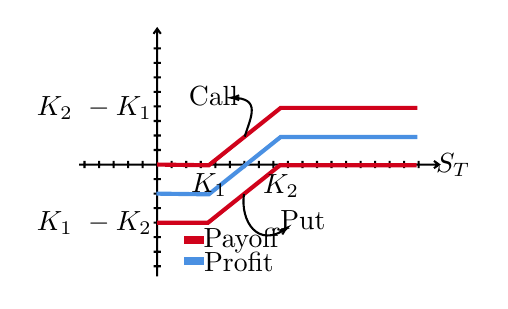
\begin{tikzpicture}[x=0.75pt,y=0.75pt,yscale=-0.35,xscale=0.35]
%uncomment if require: \path (0,363); %set diagram left start at 0, and has height of 363

%Shape: Axis 2D [id:dp28449288707577314] 
\draw  (14,195) -- (509.5,195)(121.5,8) -- (121.5,349) (502.5,190) -- (509.5,195) -- (502.5,200) (116.5,15) -- (121.5,8) -- (126.5,15) (141.5,190) -- (141.5,200)(161.5,190) -- (161.5,200)(181.5,190) -- (181.5,200)(201.5,190) -- (201.5,200)(221.5,190) -- (221.5,200)(241.5,190) -- (241.5,200)(261.5,190) -- (261.5,200)(281.5,190) -- (281.5,200)(301.5,190) -- (301.5,200)(321.5,190) -- (321.5,200)(341.5,190) -- (341.5,200)(361.5,190) -- (361.5,200)(381.5,190) -- (381.5,200)(401.5,190) -- (401.5,200)(421.5,190) -- (421.5,200)(441.5,190) -- (441.5,200)(461.5,190) -- (461.5,200)(481.5,190) -- (481.5,200)(101.5,190) -- (101.5,200)(81.5,190) -- (81.5,200)(61.5,190) -- (61.5,200)(41.5,190) -- (41.5,200)(21.5,190) -- (21.5,200)(116.5,175) -- (126.5,175)(116.5,155) -- (126.5,155)(116.5,135) -- (126.5,135)(116.5,115) -- (126.5,115)(116.5,95) -- (126.5,95)(116.5,75) -- (126.5,75)(116.5,55) -- (126.5,55)(116.5,35) -- (126.5,35)(116.5,215) -- (126.5,215)(116.5,235) -- (126.5,235)(116.5,255) -- (126.5,255)(116.5,275) -- (126.5,275)(116.5,295) -- (126.5,295)(116.5,315) -- (126.5,315)(116.5,335) -- (126.5,335) ;
\draw   ;
%Straight Lines [id:da9209384368986784] 
\draw [color={rgb, 255:red, 208; green, 2; blue, 27 }  ,draw opacity=1 ][line width=1.5]    (121.5,195) -- (192.5,196) -- (291.5,117) -- (479.5,117) ;


%Straight Lines [id:da37977537439547226] 
\draw [color={rgb, 255:red, 208; green, 2; blue, 27 }  ,draw opacity=1 ][line width=3]    (158.5,299) -- (185.5,299) ;


%Straight Lines [id:da9460733927110921] 
\draw [color={rgb, 255:red, 74; green, 144; blue, 226 }  ,draw opacity=1 ][line width=3]    (158.5,328) -- (185.5,328) ;



%Straight Lines [id:da9014316388237789] 
\draw [color={rgb, 255:red, 74; green, 144; blue, 226 }  ,draw opacity=1 ][line width=1.5]    (120.5,235) -- (192.5,236) -- (291.5,157) -- (479.5,157) ;


%Straight Lines [id:da22160788848594903] 
\draw [color={rgb, 255:red, 208; green, 2; blue, 27 }  ,draw opacity=1 ][line width=1.5]    (121.5,275) -- (191.5,275) -- (290.5,196) -- (478.5,196) ;


%Curve Lines [id:da09447744102237843] 
\draw    (241,235.5) .. controls (235.56,272.63) and (260,311.22) .. (299.3,282.88) ;
\draw [shift={(300.5,282)}, rotate = 503.13] [color={rgb, 255:red, 0; green, 0; blue, 0 }  ][line width=0.75]    (10.93,-3.29) .. controls (6.95,-1.4) and (3.31,-0.3) .. (0,0) .. controls (3.31,0.3) and (6.95,1.4) .. (10.93,3.29)   ;

%Curve Lines [id:da08283708021002456] 
\draw    (242,156.5) .. controls (250.37,129.41) and (265.05,103.78) .. (225.35,103.02) ;
\draw [shift={(223.5,103)}, rotate = 360] [color={rgb, 255:red, 0; green, 0; blue, 0 }  ][line width=0.75]    (10.93,-3.29) .. controls (6.95,-1.4) and (3.31,-0.3) .. (0,0) .. controls (3.31,0.3) and (6.95,1.4) .. (10.93,3.29)   ;


% Text Node
\draw (529,196) node  [align=left] {$\displaystyle S_{T}$};
% Text Node
\draw (193,223) node   {$K_{1}$};
% Text Node
\draw (237,300) node  [align=left] {Payoff};
% Text Node
\draw (234,329) node  [align=left] {Profit};
% Text Node
\draw (35,117) node   {$K_{2} \ -K_{1}$};
% Text Node
\draw (292,224) node   {$K_{2}$};
% Text Node
\draw (322,271) node  [align=left] {Put};
% Text Node
\draw (199,101) node  [align=left] {Call};
% Text Node
\draw (35,275) node   {$K_{1} \ -K_{2}$};


\end{tikzpicture}

